\documentclass{beamer}

\usetheme{Madrid}


\usepackage{graphicx}
\usepackage{amsmath,amssymb}
\usepackage{caption}


\DeclareMathOperator{\E}{\mathbb{E}}
\captionsetup[figure]{labelformat=empty}



\title[]{The Impact of Imputation Quality on Family Based Analysis}
\author[]{Mahdi Mir}
\institute[]{SSGAC}
\date[]{Oct 2024}


\begin{document}


\maketitle


\begin{frame}{What is imputation?}
      \begin{itemize}
            % firs I gibve a brief introduction to imputation
            \item Imputation is a process in which we predict the genotypes that are not directly observed.
            \item We use the information from the observed genotypes to predict the unobserved genotypes.
            \item With the help of a reference panel we can predict the genotypes that are not directly observed.
      \end{itemize}
\end{frame}

\begin{frame}{What is imputation?}
      \begin{figure}
            \centering
            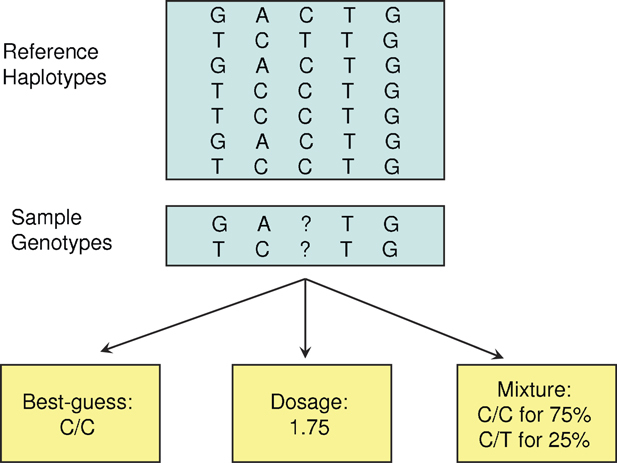
\includegraphics[width= .7\textwidth]{fig/mfig001-2.jpg}
            \caption{Source: Zheng et al. (2011)}
      \end{figure}
\end{frame}

\begin{frame}{Why Imputation?}
      \begin{itemize}
            \item Imputation is used to increase the number of SNPs that are available for analysis.
            \item Imputation is used in GWAS to increase the power of the study.
      \end{itemize}
\end{frame}

\begin{frame}{Motivation}
      \begin{itemize}
            \item We are concerned that low-quality imputed genotypes may not work for family based analysis. % and maybe for other types of analysis
            \item Family-based research designs rely on special properties of family data that might not be preserved in low quality imputed genotypes.
            \item E.g.: In theory by the Mandellian laws we expect the correlation between sibling pairs and parent-offspring pairs genotypes to be 0.5.
            % but this is not true for low quality imputed genotypes.
      \end{itemize}
\end{frame}

\begin{frame}{Introduction}
      \begin{itemize}
            % and I am going to show that in this presentation.
            \item We are going to show some correlation analysis between sibling pairs and parent-offspring pairs.
            \item We show the low quality imputed genotypes correlation deviates from the theoretical expectations.
            % not all imputed genotypes are bad its more lower quality imputed genotypes might be bad.
            % this is imporant because some studies have used low quality imputed genotypes in their analysis. and that might not be a good idea.
            \item E.g.: Howe et.al (2022) Sib-GWAS paper used low quality imputed SNPs in its analysis.
      \end{itemize}
\end{frame}

\begin{frame}{Correlation Analysis on the Imputed Data}
      \begin{itemize}
          \item In theory, we should see 0.5 correlation between both full-sibling and parent-offspring pairs genotypes.
          \item So if the imputed genotypes is high quality imputed then we should see the distribution of correlations to be concentrated around the half.
          \item Expectation: we would expect more deviation for low quality SNPs from the theoretical expectation.
      \end{itemize}
\end{frame}

% in this part we have some nice figures to show to you that conveys the whole point we are going to show.
% there are some really minute and small steps that I took that I didn't mention them here because it gets too technical but just 
% to say each of these steps as you know when you are writng and testing and developing the code every step could be 
% Challening, but addressing each of them would be too much technical talk.

% mention the repos that I created so far

\begin{frame}{Sample}
      \begin{itemize}
            \item UKB Imputed Data.
            % we have a sample of around 19K sibling pairs and 4K parent-offspring pairs. in this analysis in the UK Biobank data.
            \item \(19K\) of sibling pairs.
            \item \(4K\) parent-offspring pairs.
            % \item For each info score we selected 1000 SNPs randomly from the enitre genome.
      \end{itemize}
\end{frame}

\begin{frame}{Correlations Distribution - Full Siblings}
      \begin{columns}
            \begin{column}{0.5\textwidth}
                  \centering
                  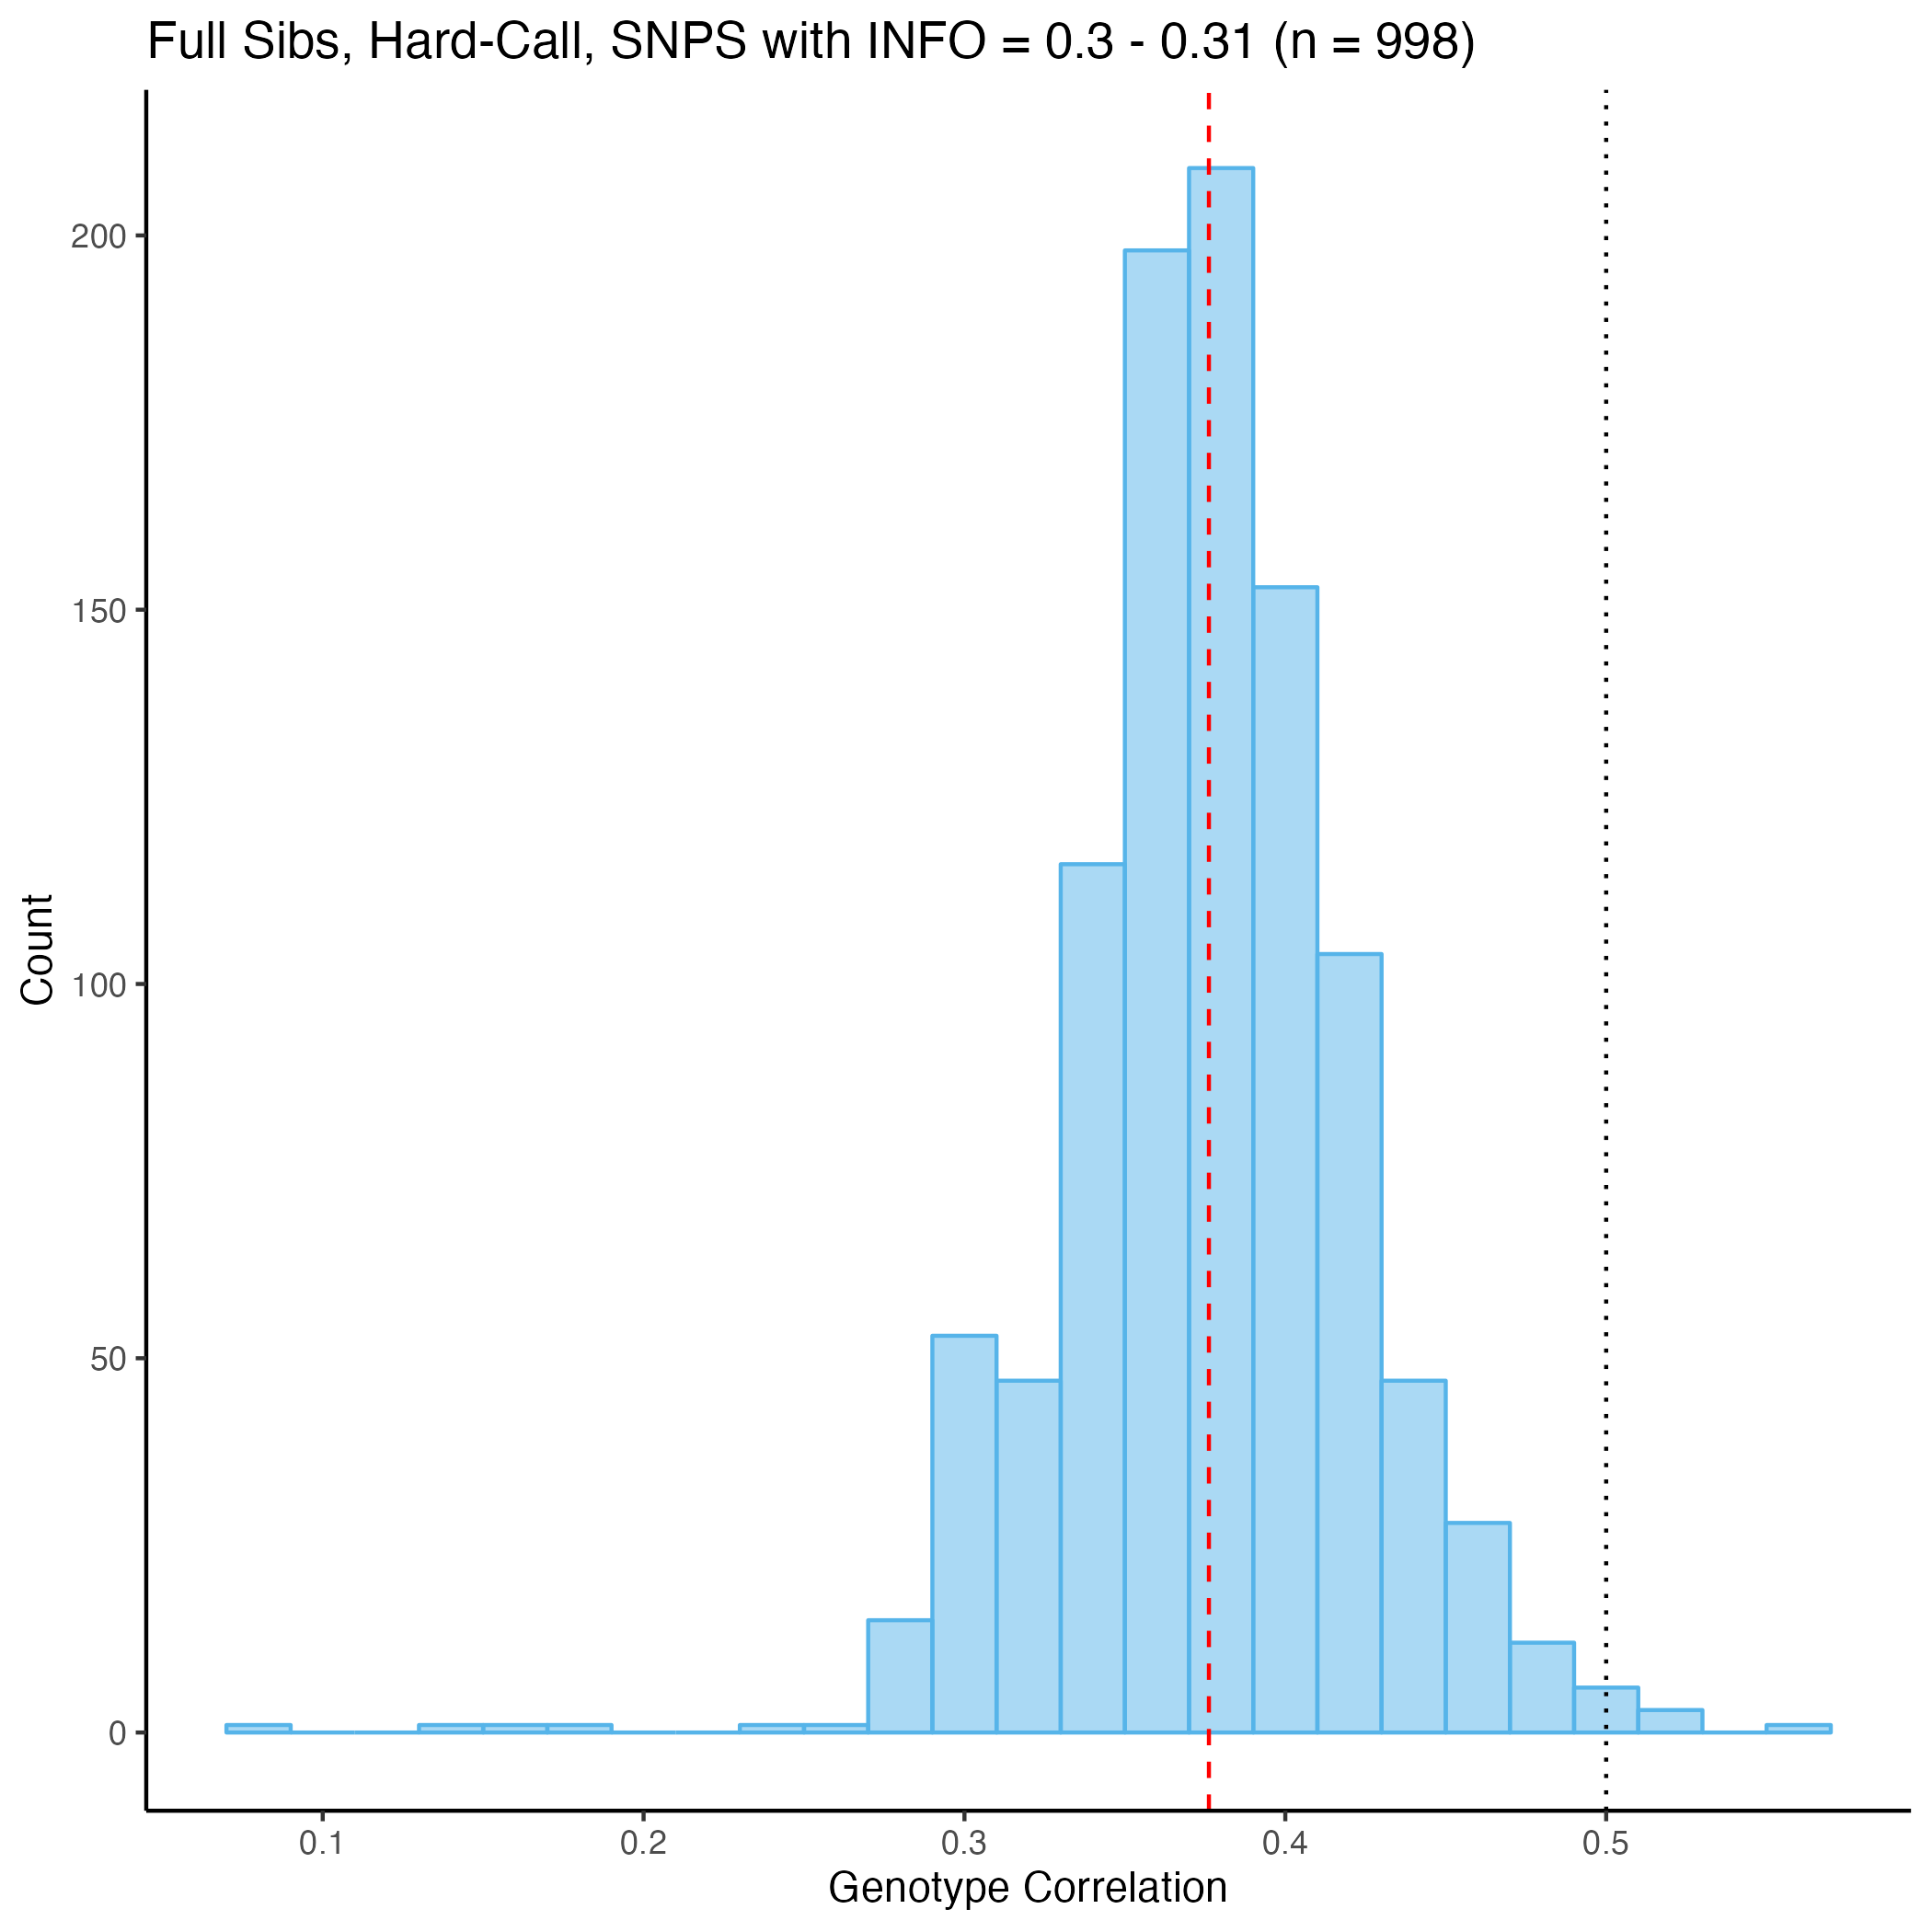
\includegraphics[width= \textwidth]{fig/FS-HC-i30.png}
                  \captionof{figure}{Low Quality Imputed SNPs}
              \end{column}
            \begin{column}{0.5\textwidth}
                \centering
                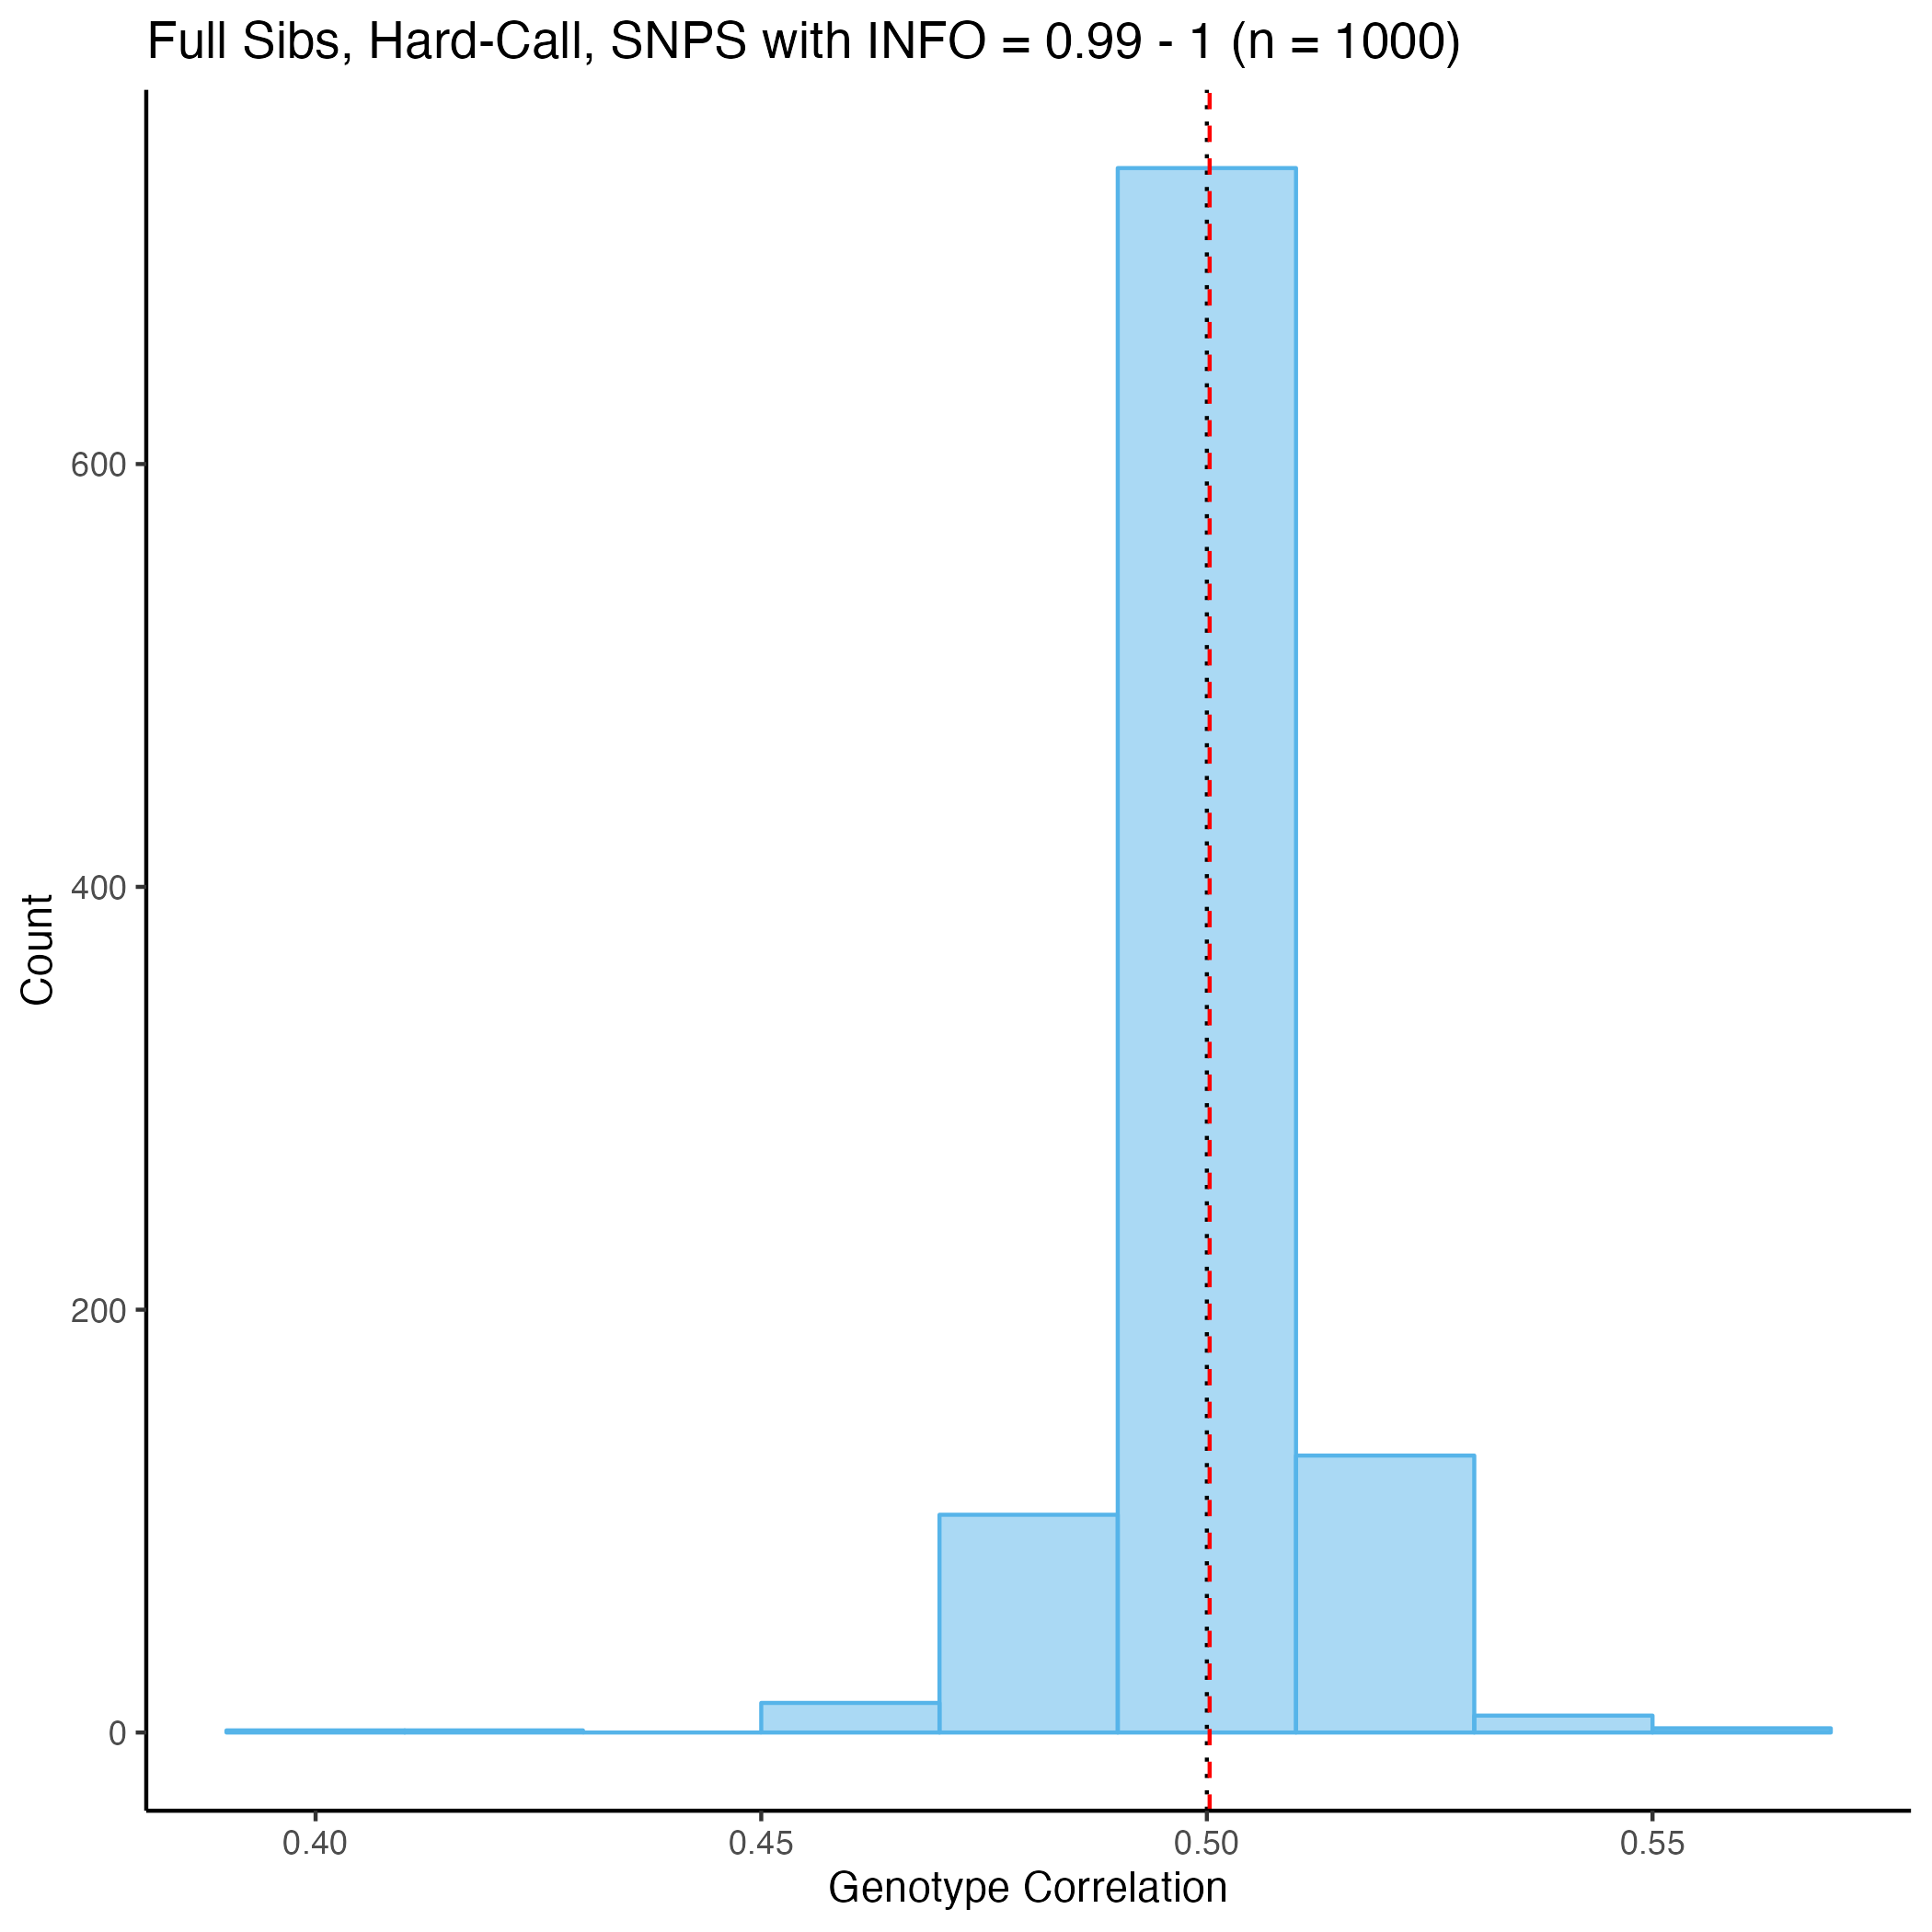
\includegraphics[width= \textwidth]{fig/FS-HC-i99.png}
                \captionof{figure}{High Quality Imputed SNPs}
            \end{column}
        \end{columns}       
\end{frame}

\begin{frame}{Correlations Distribution - Parent-Offspring}
      \begin{columns}
            \begin{column}{0.5\textwidth}
                  \centering
                  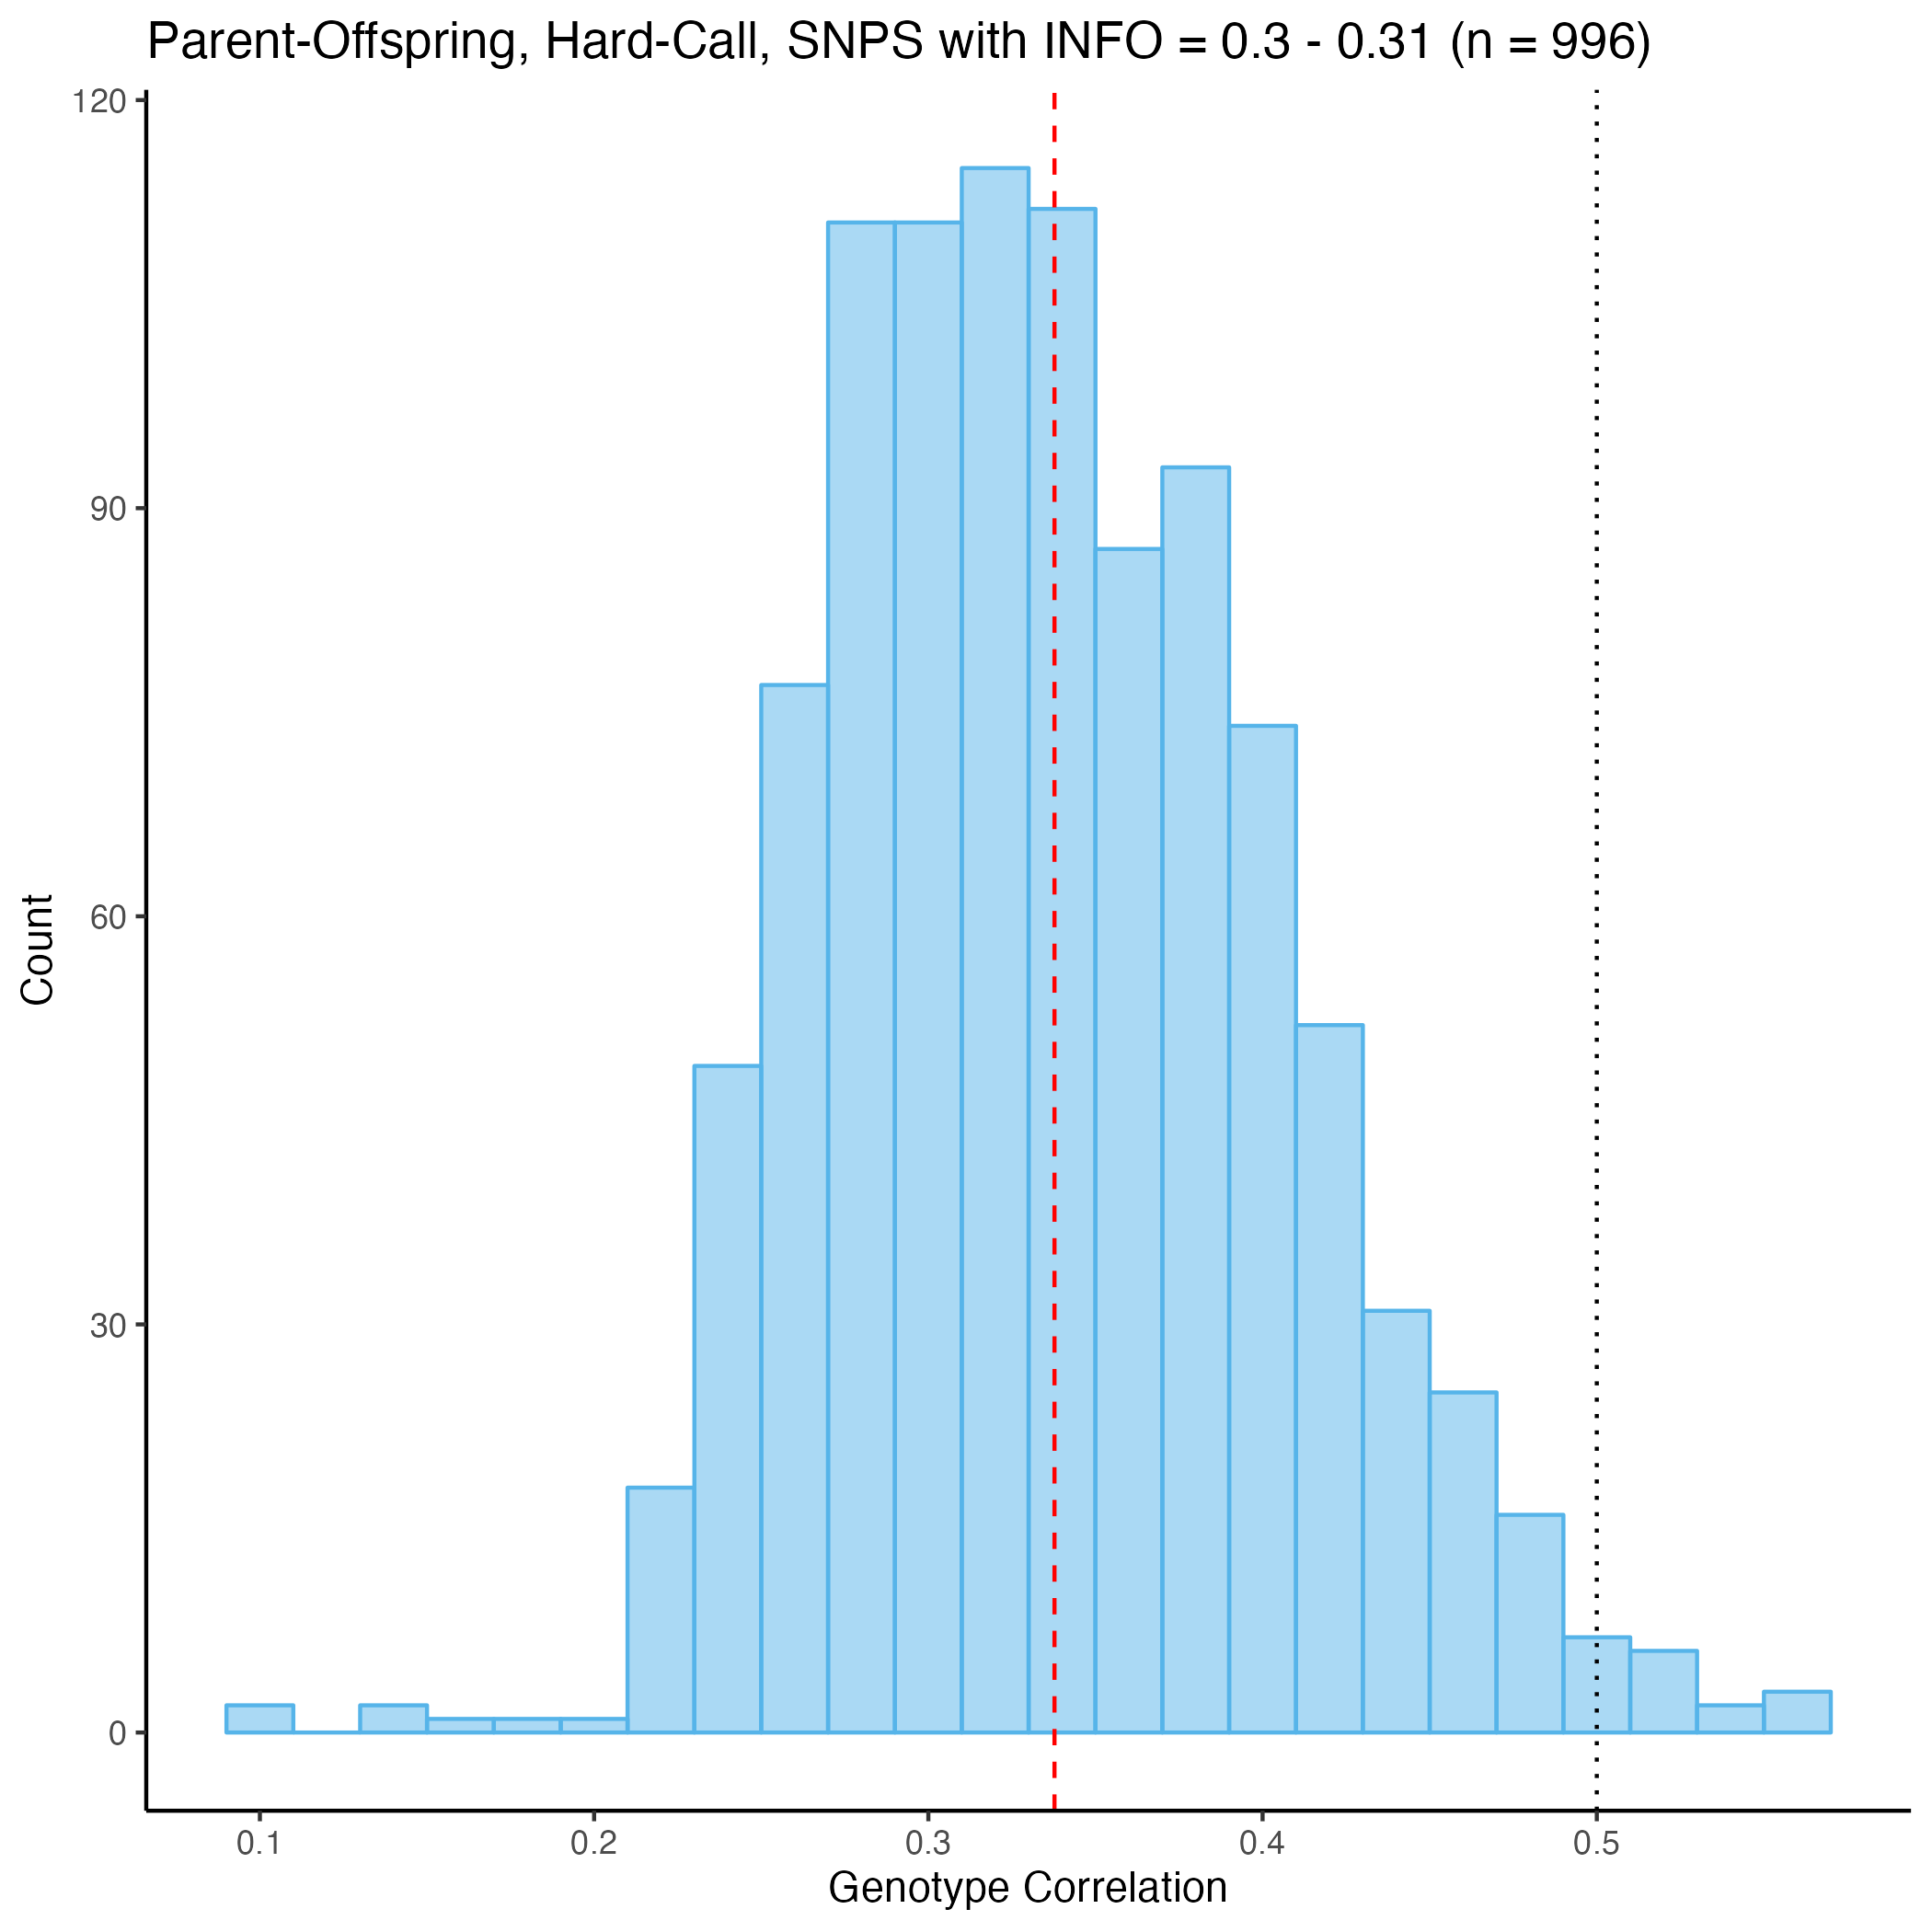
\includegraphics[width= \textwidth]{fig/PO-HC-i30.png}
                  \captionof{figure}{Low Quality Imputed SNPs}
              \end{column}
            \begin{column}{0.5\textwidth}
                \centering
                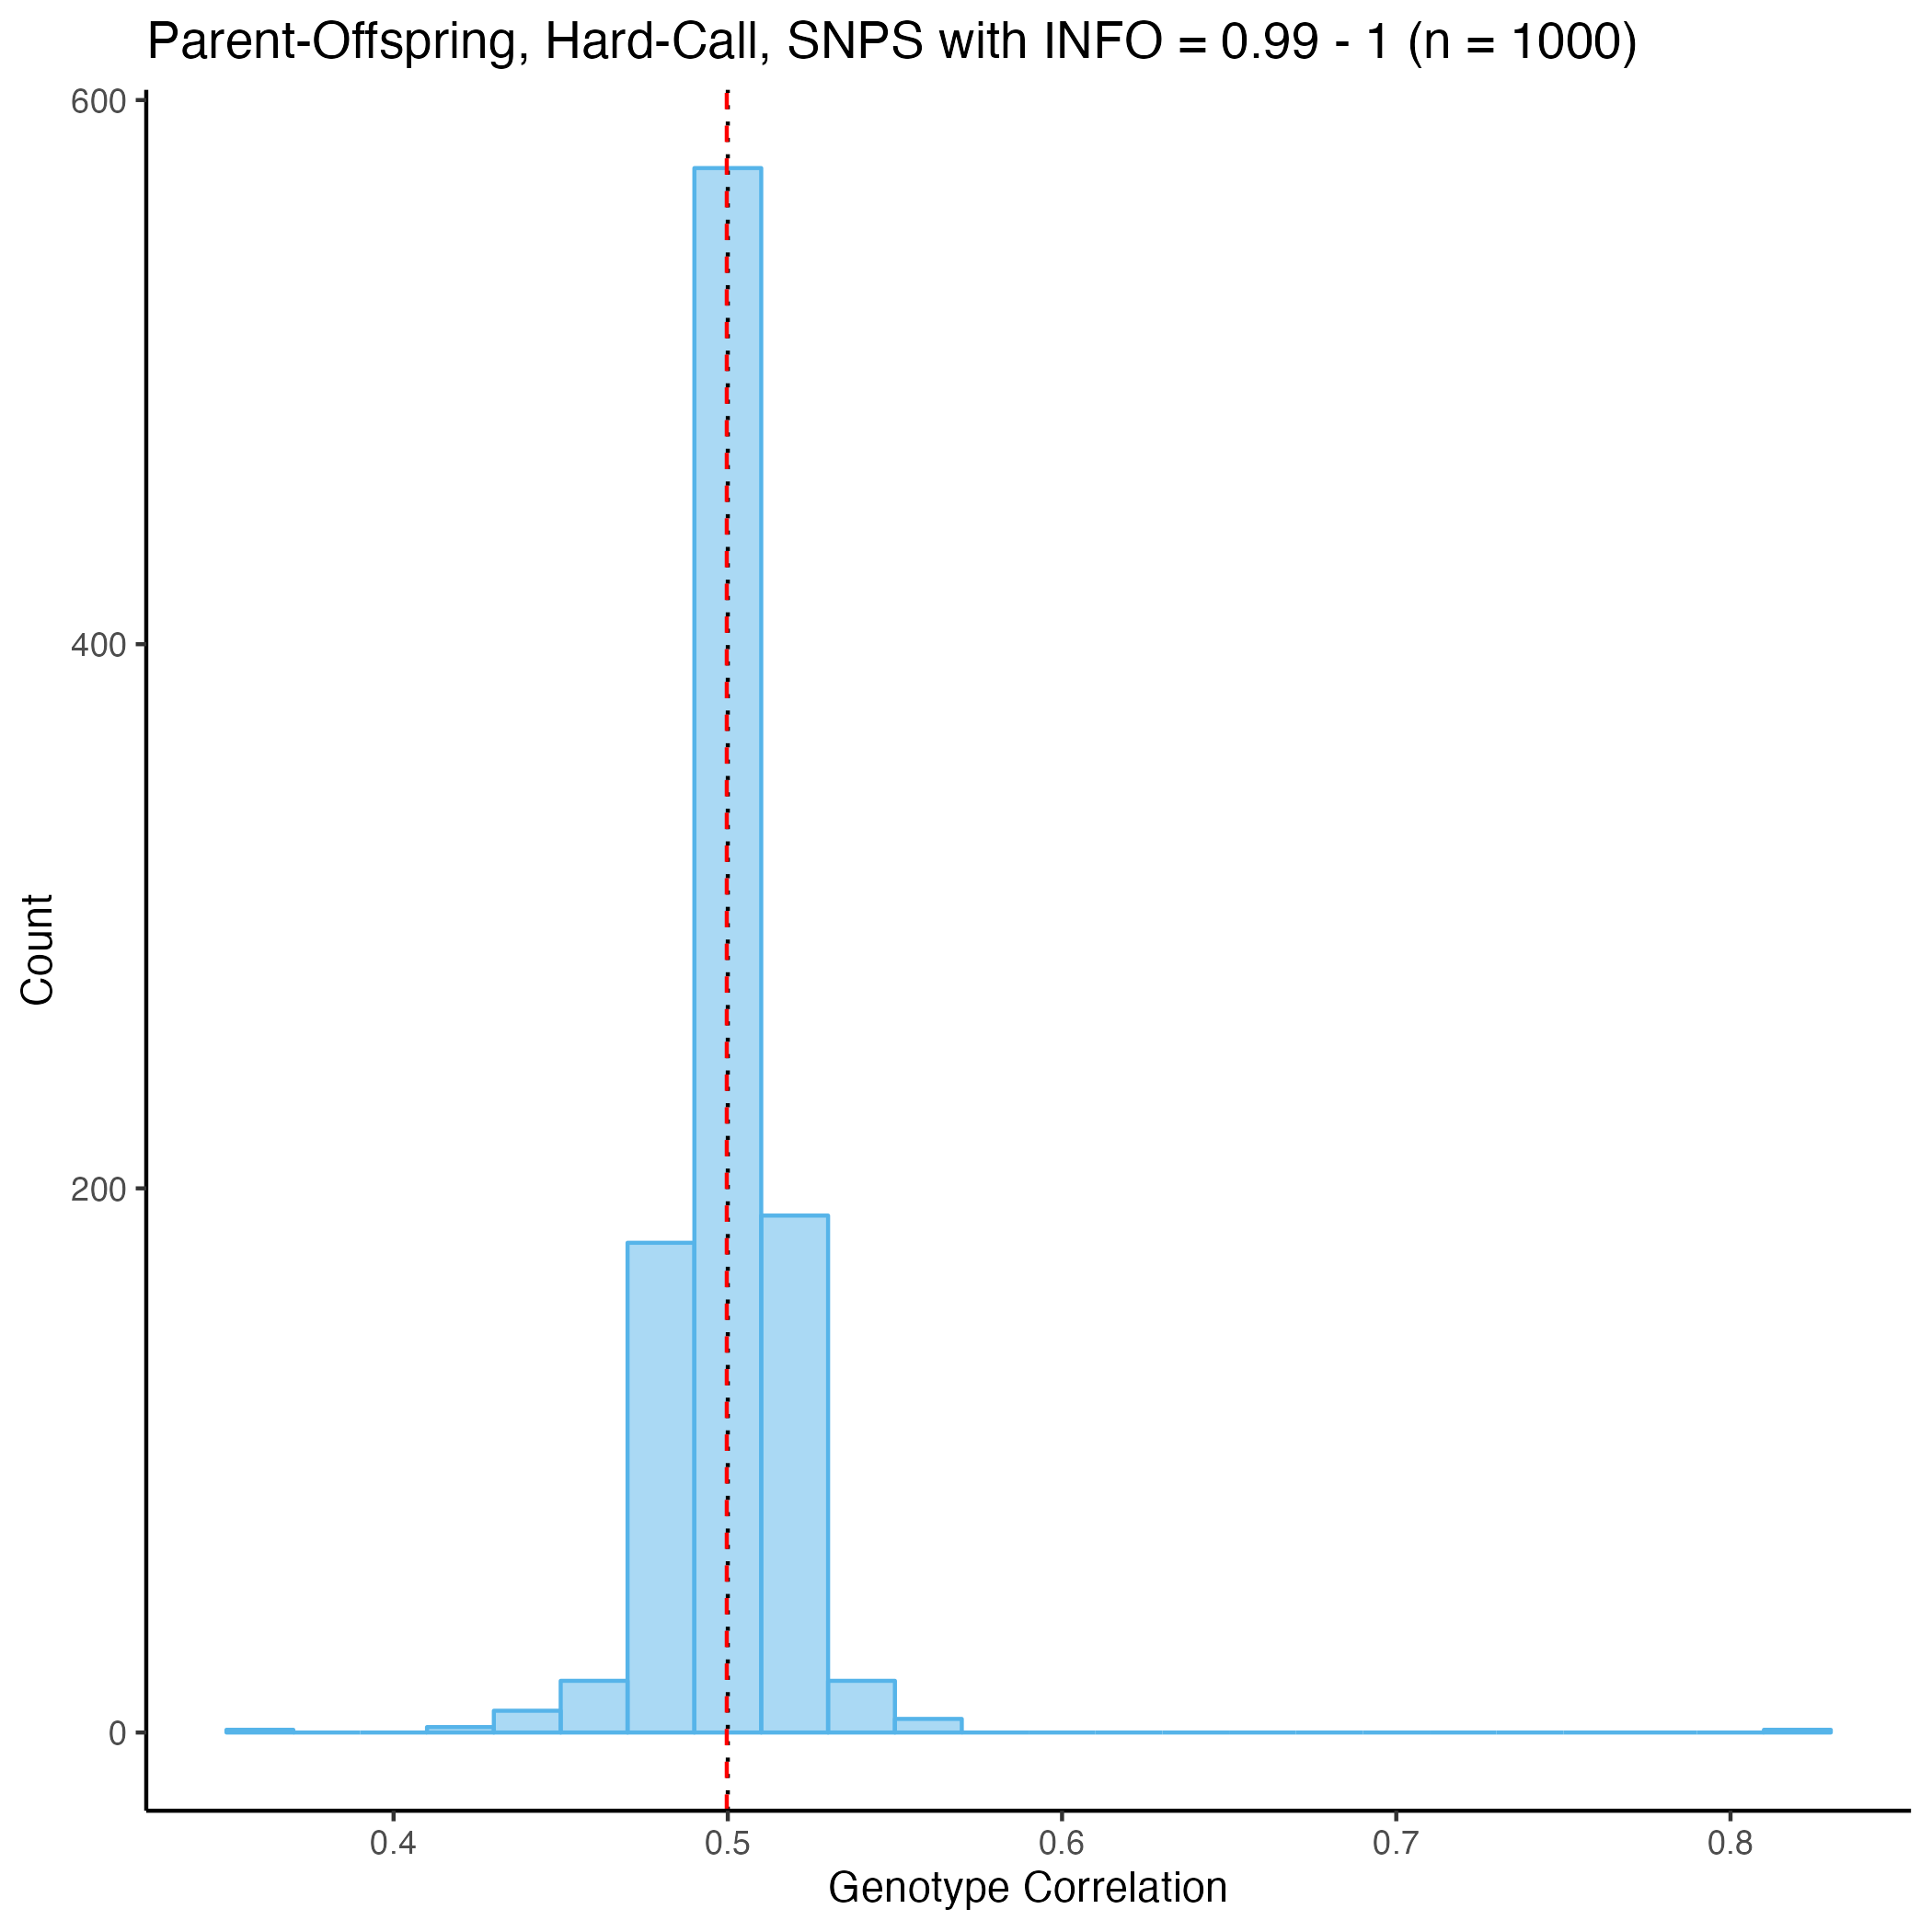
\includegraphics[width= \textwidth]{fig/PO-HC-i99.png}
                \captionof{figure}{High Quality Imputed SNPs}
            \end{column}
        \end{columns}       
\end{frame}

\begin{frame}{Mean Genotype Correlation}
      \centering
      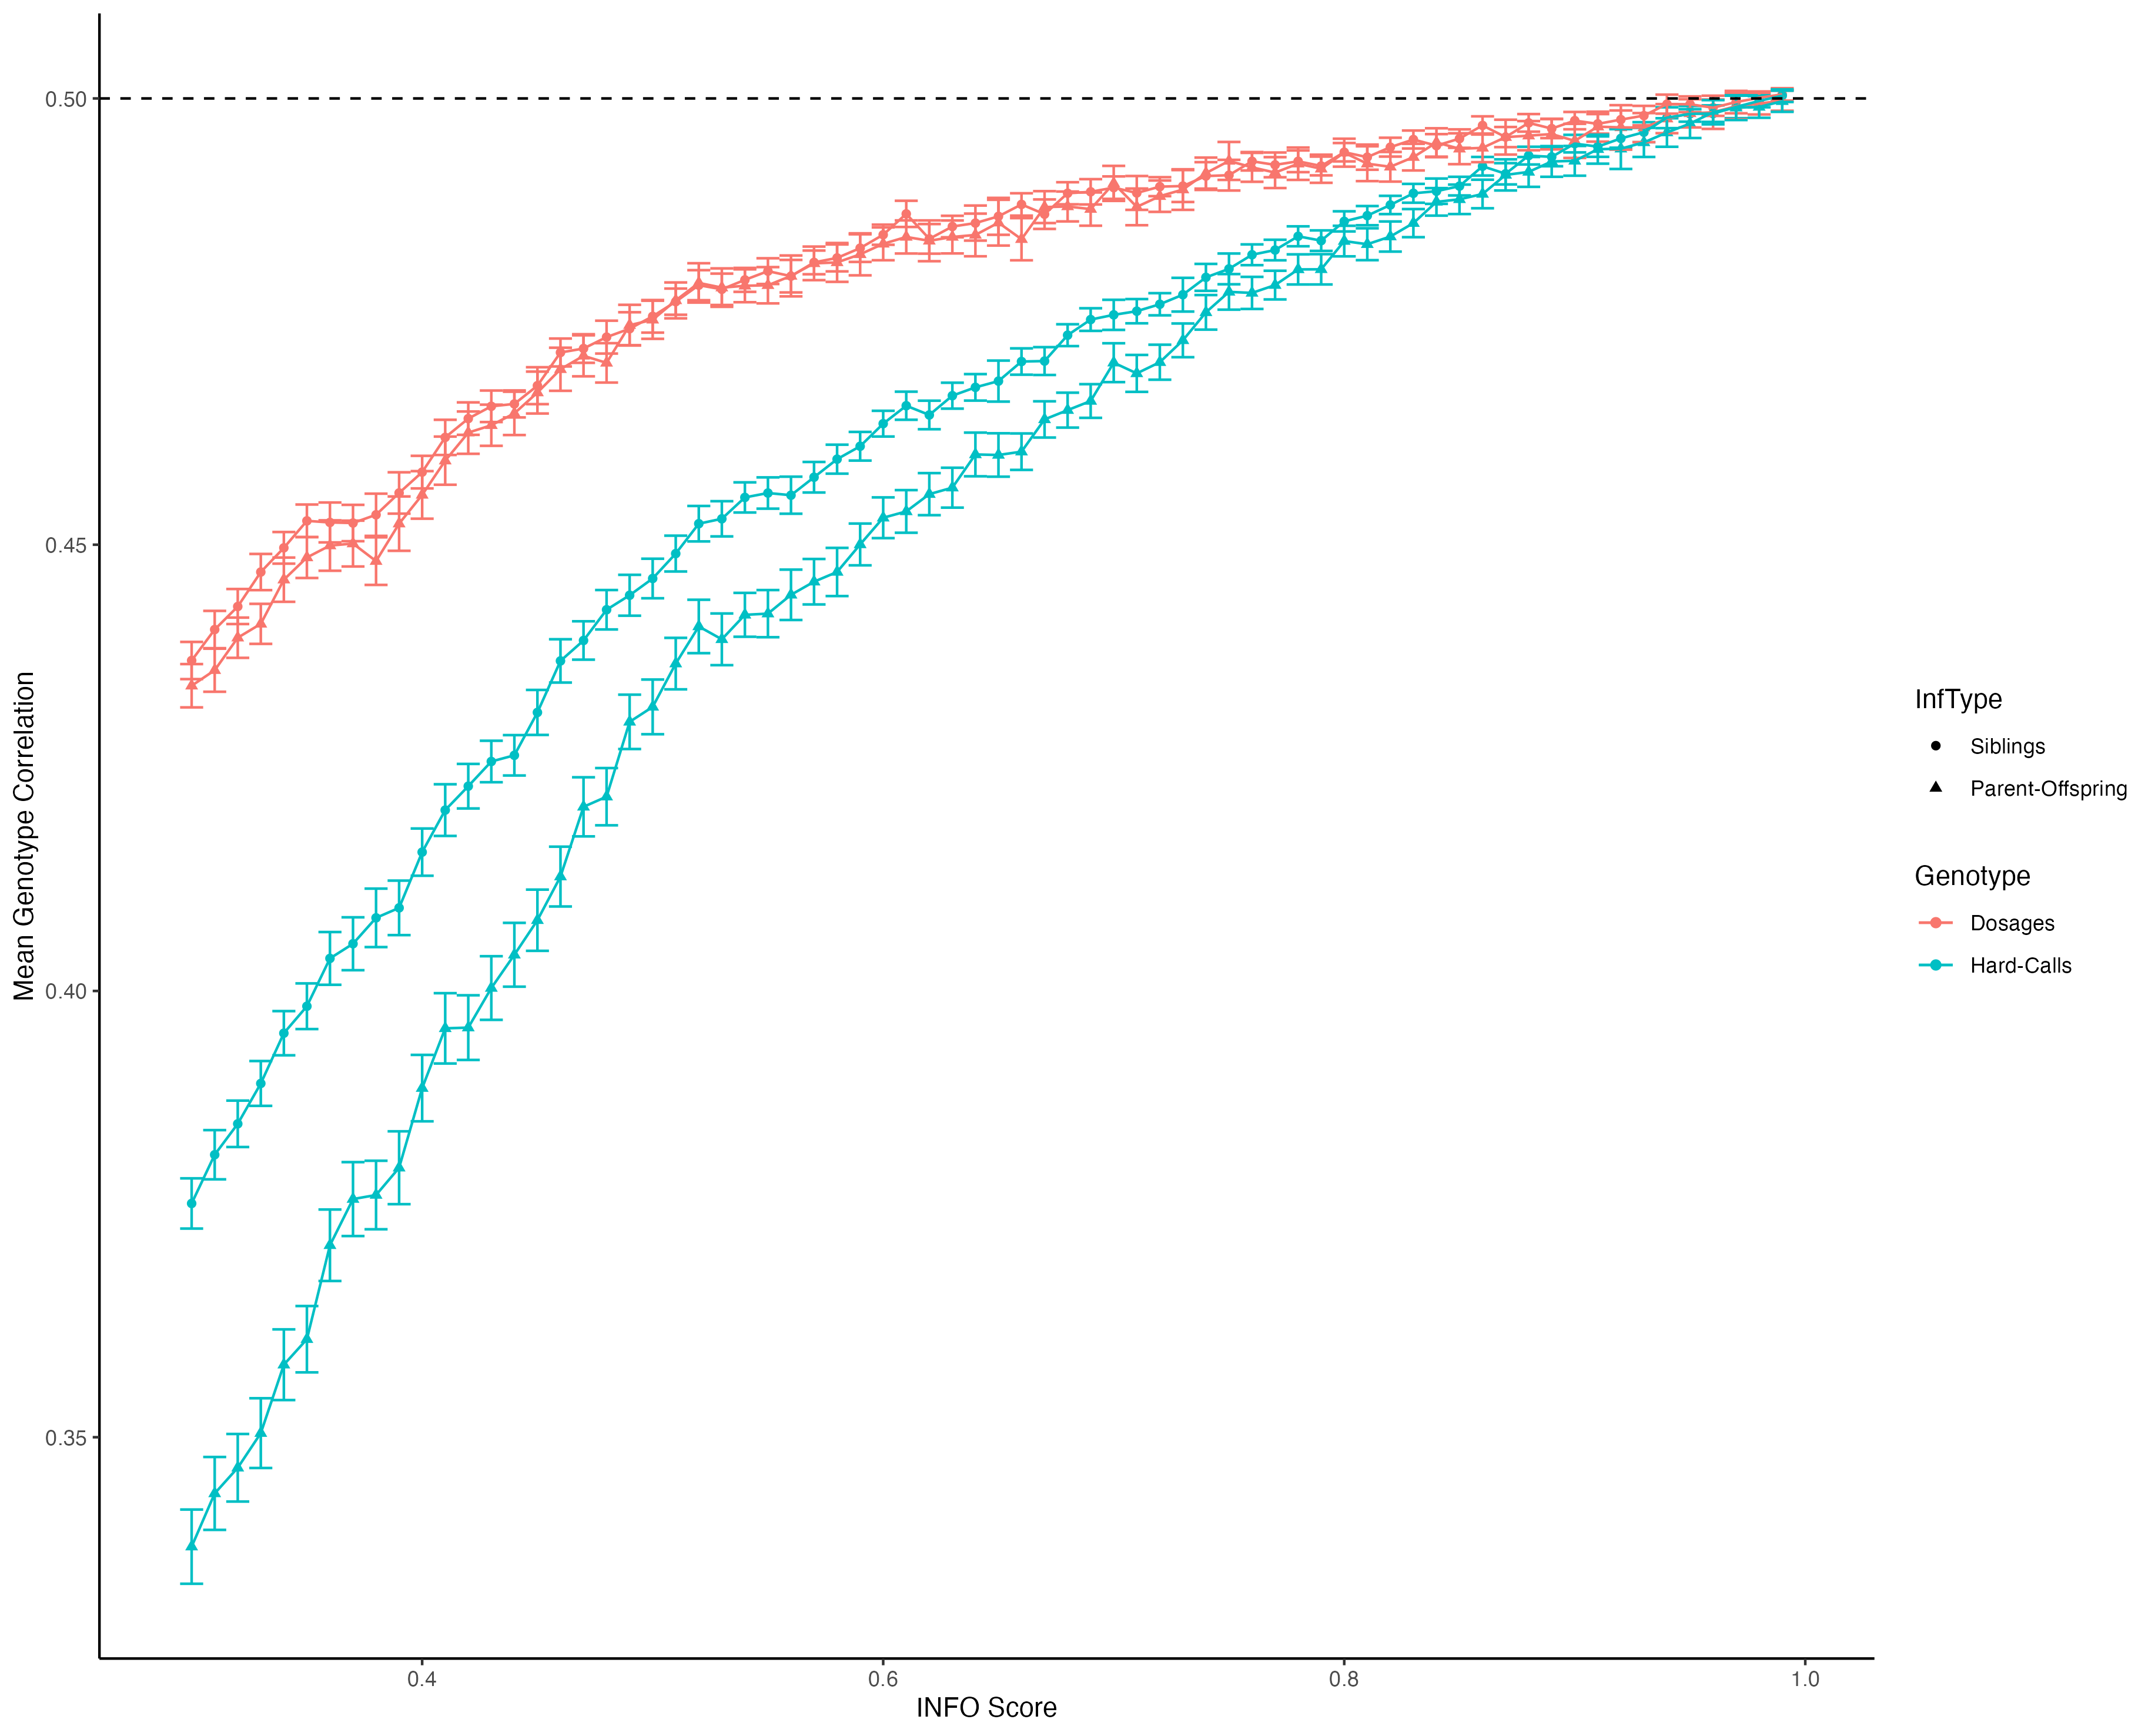
\includegraphics[width=.83\textwidth]{fig/mean_gt_corr_v2.png}
\end{frame}

\begin{frame}{Correlation Analysis Conditional on IBD states}
      % the genome is the same for that siblings pairs. So they are inheriting the same from both parents.
      % when IBD is 2 it means that in that part of the genome both paternal & maternal side of
      \begin{itemize}
            \item Suppose \(i\) and \(j\) are siblings. Then in theory we have
      \end{itemize}
      \[
            Corr(G_i, G_j | IBD = 0) = 0
      \]
      \[
            Corr(G_i, G_j | IBD = 1) = 0.5
      \]
      \[
            Corr(G_i, G_j | IBD = 2) = 1
      \]
\end{frame}

\begin{frame}{Mean Genotypes (info score)}
      \begin{figure}
            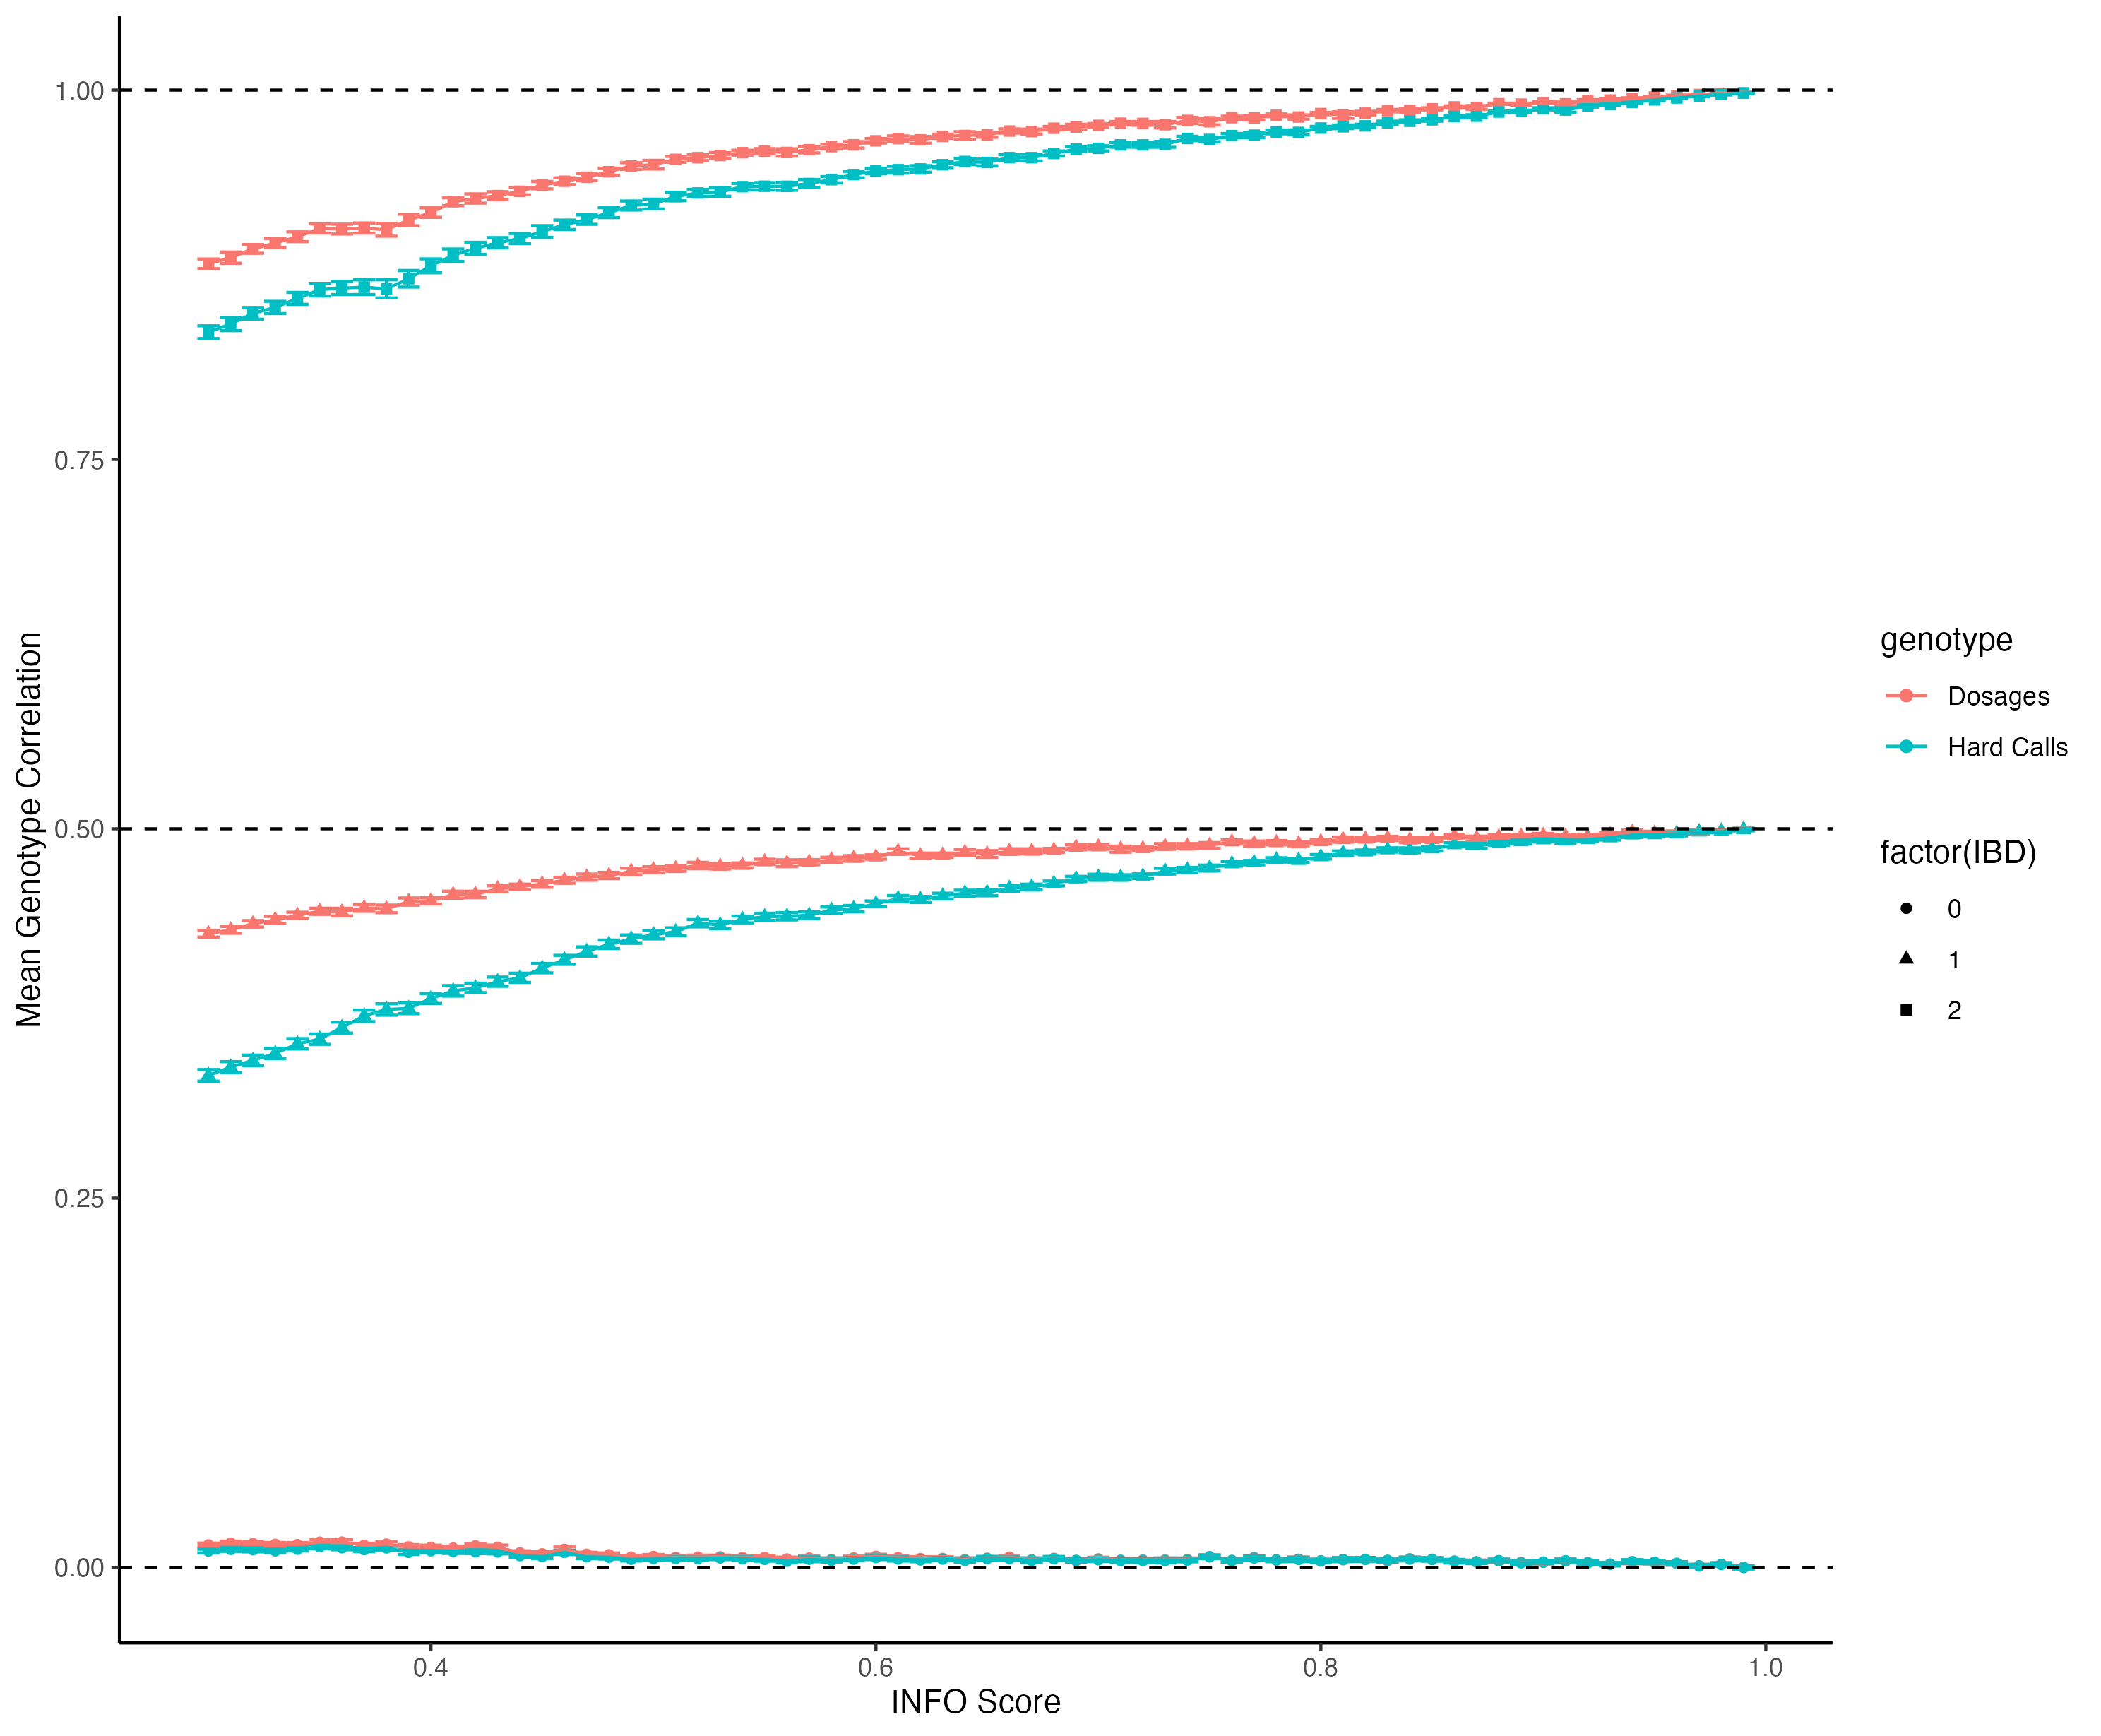
\includegraphics[width= .80\textwidth]{fig/mean_gt_by_ibd.png}
      \end{figure}
\end{frame}

\begin{frame}[plain]

      \huge{Thank You!}

\end{frame}

\end{document}